Representative prediction examples are shown in Figures~\ref{fig:qual1}–\ref{fig:qual3}. Ground-truth keypoints are drawn in green, while model predictions are overlaid in red. These cases illustrate common failure modes: symmetric confusion (left/right swaps), gross joint misplacement, and inability to handle occlusion or multi-person scenes.

\begin{figure}[!htbp]
  \centering
  %—— 子图 (a) ——%
  \subcaptionbox{Cooking scenario: ground truth vs.\ prediction.%
    \label{fig:qual1}}[.3\textwidth]{%
    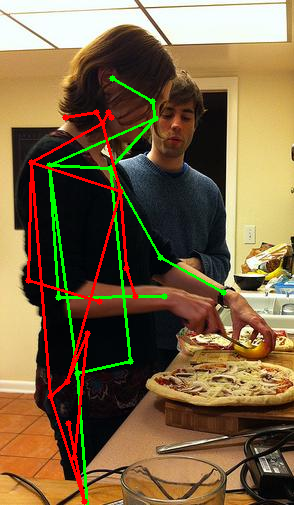
\includegraphics[width=.2\textwidth]{figures/qualitative_case1.png}%
  }\hfill
  %—— 子图 (b) ——%
  \subcaptionbox{Seated pose: ground truth vs.\ incoherent tangle.%
    \label{fig:qual2}}[.3\textwidth]{%
    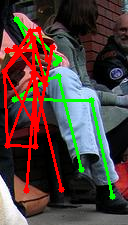
\includegraphics[width=.2\textwidth]{figures/qualitative_case2.png}%
  }\hfill
  %—— 子图 (c) ——%
  \subcaptionbox{Standing frontal pose: left/right swap.%
    \label{fig:qual3}}[.3\textwidth]{%
    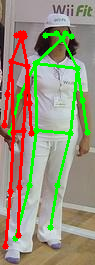
\includegraphics[width=.13\textwidth]{figures/qualitative_case3.png}%
  }

  \caption{Representative qualitative failure cases (green = GT, red = pred).}
  \label{fig:qualitative_all}
\end{figure}